% !TEX root = ../main.tex

%\begin{frame}{Tripod Handle Controls}
%	\begin{columns}[T,onlytextwidth]
%	\column{0.5\textwidth}
%	\begin{figure} 
%		\centering
%		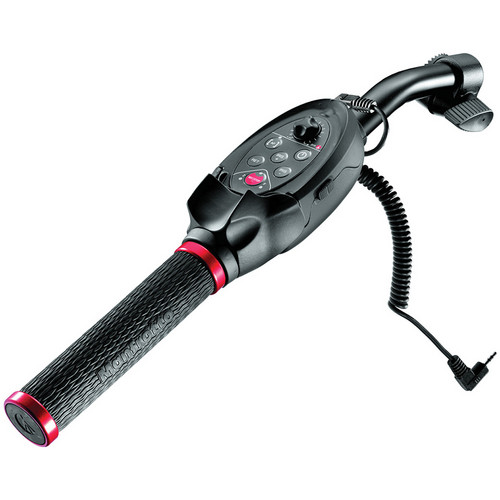
\includegraphics[width=0.7\textwidth]{images/tripod-handle.jpeg}
%		\caption{Tripod Handle}
%	\end{figure}
%
%	\column{0.5\textwidth}
%	Beware: various models in use.
%	\begin{description}
%		\item[Zoom Control] lever above red ring
%		\item[Red Button] Start/stop recording, don't touch
%		\item[Other Buttons] markings on the handle
%   \end{description}
%	\end{columns}
%\end{frame}

\begin{frame}{Tripod}
	\begin{columns}[T,onlytextwidth]
	\column{0.4\textwidth}
	\begin{figure} 
		\centering
		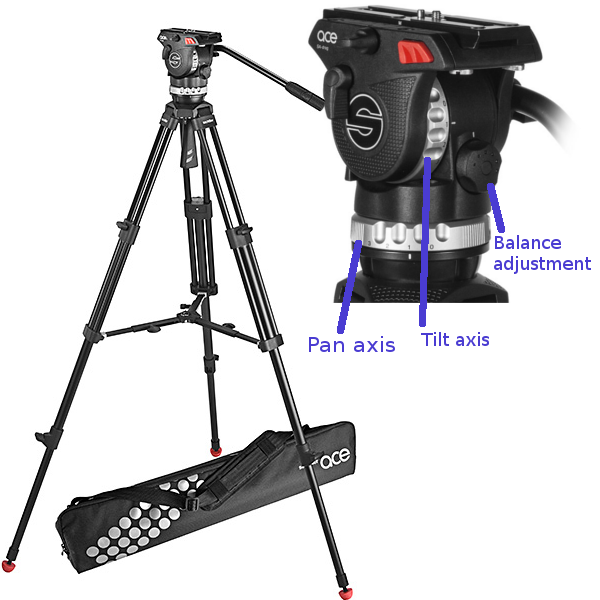
\includegraphics[width=0.9\textwidth]{images/tripod-complete.png}
		\caption{Tripod}
	\end{figure}
	
	\column{0.6\textwidth}
	\begin{itemize}
			\item Should be level - check the water bubble.
			\item Variable brakes - can be adjusted to your needs.
			\item Tilt axis should be balanced, so that the camera doesn't tilt up or down on its own.
			\item Pan axis is needed all of the time. Set it so you can do smooth pans all over the stage.
		\end{itemize}
		\metroset{block=fill}
		\begin{alertblock}{Alert}
			Alert the A/V-Technician if something's wrong or misplaced.
		\end{alertblock}
	\end{columns}
\end{frame}

\begin{frame}{SD-Card Recording}
		\begin{itemize}
			\item Two SD-Cards in every Camera
			\item Backup Recording
			\item Turn on Recording before first shift in the morning -> Red Dot somewhere in the Display.
			\item Control Recording Time remaining. 
		\end{itemize}
		\metroset{block=fill}
		\begin{alertblock}{Alert}
			Alert the A/V-Technician if something's wrong or not running.
		\end{alertblock}
\end{frame}
